\chapter{Descripción metodológica del trabajo}

El proceso de trabajo llevado a cabo para el presente proyecto, así como sus tiempos de planificación y ejecución, se exponen aquí desde dos perspectivas: la del proyecto global desde su concepción (investigación, contactos, visitas al GME, etc.), y la del desarrollo del software en sí, que lleva su propio tiempo y calendario. 

\section{El proyecto en su conjunto}



Proyecto en su conjunto:

1. Contacto con los responsables del GME y la universidad de CLM. FOTO CON JULIO Y SYLVIA, 
2. Investigación sobre los sintetizadores modulares, y los de EMS en particular
3. Inicio del desarrollo de la app
3. fotografiado exhaustivo del Synthi 100
4. Inicio de desarrollo de la GUI
5. Diversas sesiones de pruebas de módulos y testeos . FOTO DE VISITA AL GME CON LA APLICACIÓN
6. Elaboración de la memoria



Tiempos del desarrollo de la app

Es aquí donde se ha invertido la mayor parte del tiempo.
Repositorio git tiene la historia, planteamientos fallidos, giros, decisiones importantes, En total 328 commits.
link al vídeo de gource de la aplicación.


\begin{figure}
	\centering
%	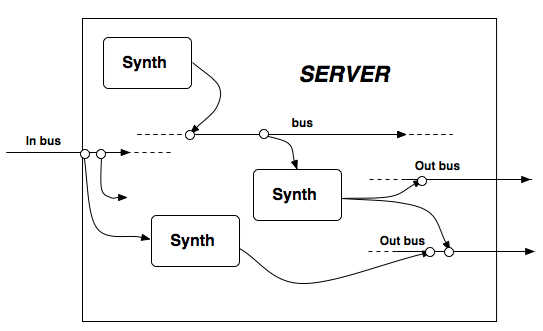
\includegraphics[width=0.7\textwidth]{images/sc_server}
	\caption[]{}
	\label{fig:}
\end{figure}
